\documentclass{beamer}

\usepackage[T1,T2A]{fontenc}
\usepackage[utf8]{inputenc}
\usepackage[russian, english]{babel}

\usepackage{amsmath, amsfonts, amsthm, amscd}
%\usepackage{graphics}
\usepackage{graphicx}
\usepackage[matrix,arrow,curve]{xy}
%\usepackage{multicol}

%----------------------------------------------------

\newtheorem{problemR}{Проблема}
\newtheorem{aim}{Цель}


\newtheorem{construction}{Construction}
\newtheorem{problems}{Problems}
\newtheorem{conjecture}{Conjecture}
\newtheorem{question}{Question}

\mode<presentation>
\usetheme{Madrid}

\title{}
\date{2021}
\author{Константин Амеличев}


\begin{document}



\begin{frame}
\begin{center}


{\large \scshape

\bigskip

\bigskip

3d-Renderer с нуля

\bigskip
\bigskip
\bigskip
\bigskip
\bigskip
\bigskip
}



Выполнил: Амеличев Константин, ПМИ 191\\
\bigskip
Научный руководитель: Трушин Дмитрий Витальевич, ФКН ВШЭ


\end{center}
\end{frame}

\begin{frame}

\frametitle{Цель работы}

Разработка библиотеки для отрисовки объектов из 3d-пространства

\bigskip

Из пререквизитов~--- только отрисовка пикселей на экране.

\end{frame}

\begin{frame}

\frametitle{Поставленные задачи}

\begin{itemize}
\item Изучение теории
\item Сборка пайплайна
\item Создание приложения
\item Тестирование
\item Документация
\end{itemize}

\end{frame}


\begin{frame}

\frametitle{Изучение теории}

\begin{itemize}

\item Однородные координаты для работы с 3d-пространством
\begin{itemize}
\item $\begin{pmatrix} x \\ y \\ z \\ w \end{pmatrix} \iff \begin{pmatrix} \frac{x}{w} \\ \frac{y}{w} \\ \frac{z}{w} \\ 1 \end{pmatrix} \iff \begin{pmatrix} \frac{x}{w} \\ \frac{y}{w} \\ \frac{z}{w} \end{pmatrix}$
\item Расширяется возможность линейных отображений
\end{itemize}
\item Повороты и сдвиги
\item Проективное преобразование
\item Работа с матрицами

\end{itemize}


\end{frame}

\begin{frame}
\frametitle{Pipeline}

\begin{center}
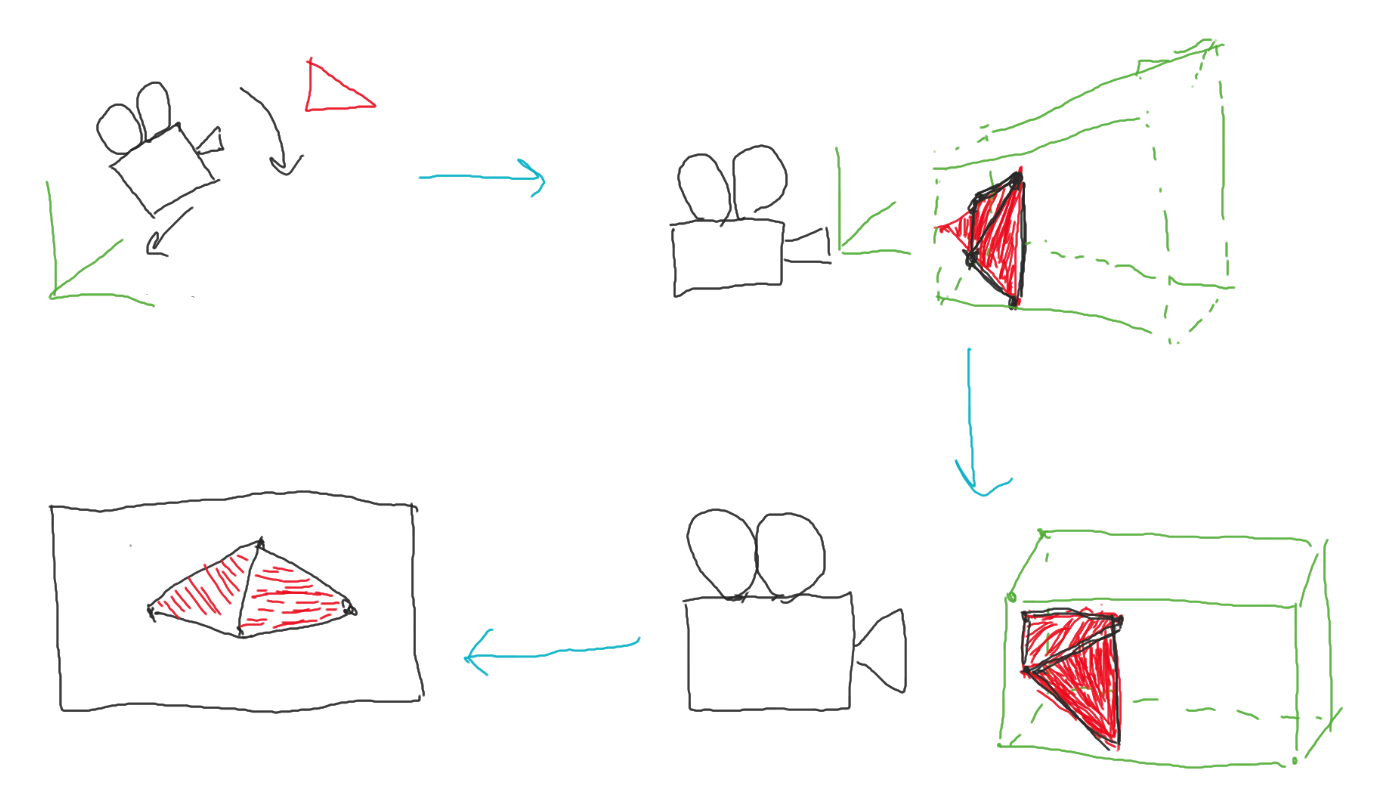
\includegraphics[width=0.6 \linewidth]{presentation_pipeline.png}
\end{center}
\begin{itemize}
\item Перенос объекта в систему координат камеры.
\item Клиппинг (выбор объектов для отображения).
\item Проективное преобразование
\item Растеризация
\end{itemize}

\end{frame}

\begin{frame}
\frametitle{Алгоритмическая часть: Клиппинг}

\begin{center}
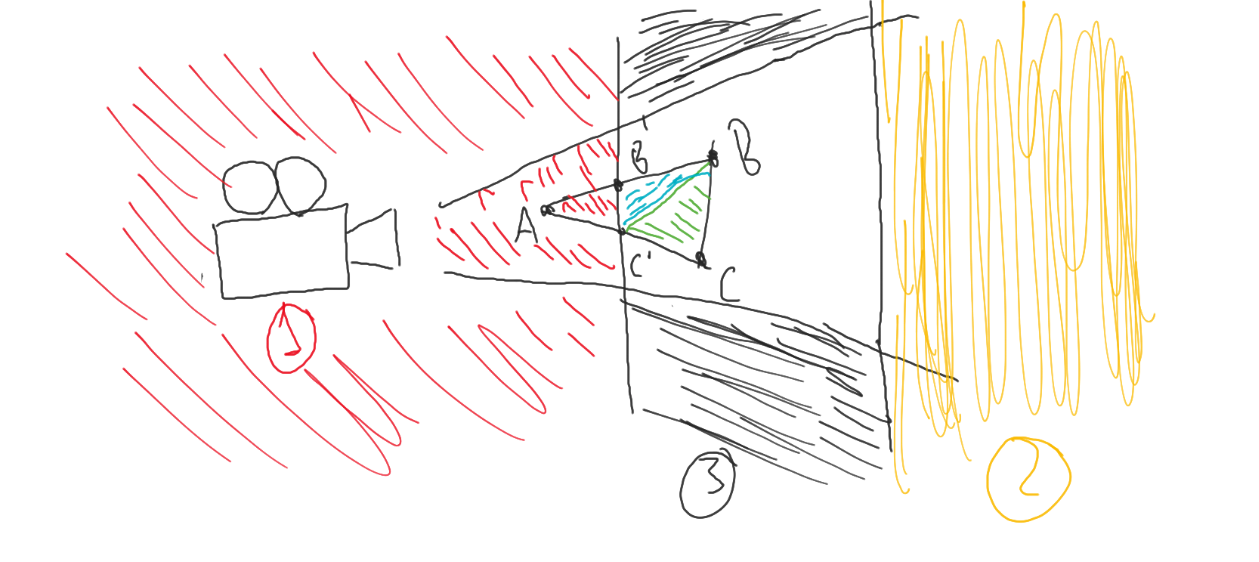
\includegraphics[width=\linewidth]{clipping.png}
\end{center}
Отсекаем невидимые области:
\begin{enumerate}
	\item Отсекается клиппингом, за передней плоскостью
	\item Слишком большая $z$-value
	\item За границами 2д-экрана
\end{enumerate}
\end{frame}

\begin{frame}
\frametitle{Алгоритмическая часть: Растеризация}

\begin{center}
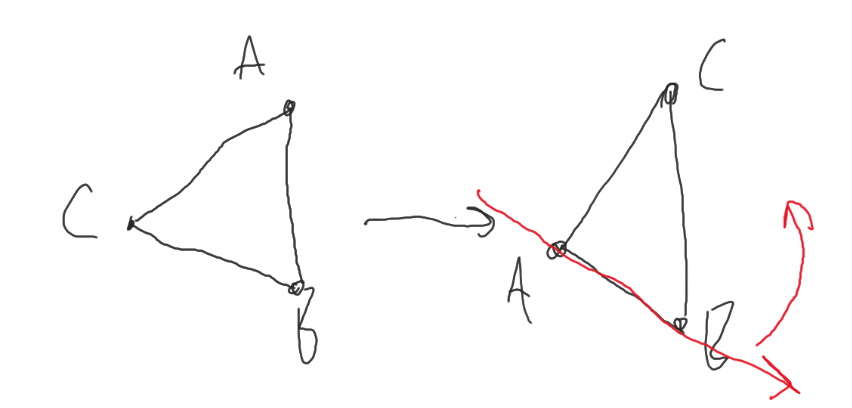
\includegraphics[width=\linewidth]{sort_triangle_1.png}
\end{center}

Теперь можно легко выделить вертикальную полосу в треугольнике.
\end{frame}

\begin{frame}
\frametitle{Алгоритмическая часть: Растеризация}

\begin{center}
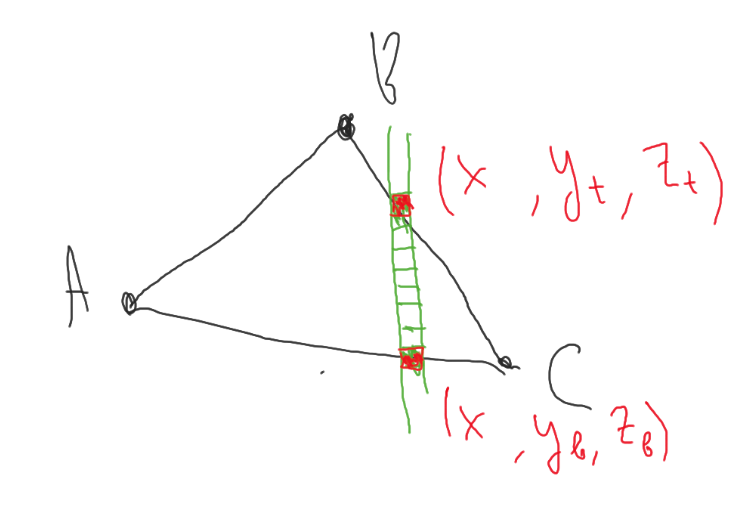
\includegraphics[width=0.5 \linewidth]{sweepline_1.png}
\end{center}

\begin{enumerate}
\item Нахождение $y_b, y_t$~--- пересечение вертикальной прямой и треугольника
\item Нахождение $z_b, z_t$~--- перенос двумерной точки $(x, y)$ обратно в трехмерное пространство.
\item Нахождение $z$-value внутри~--- линейно относительно  $z_b, z_t$
\end{enumerate}

\end{frame}


\begin{frame}
\frametitle{Схема взаимодействия}

\begin{center}

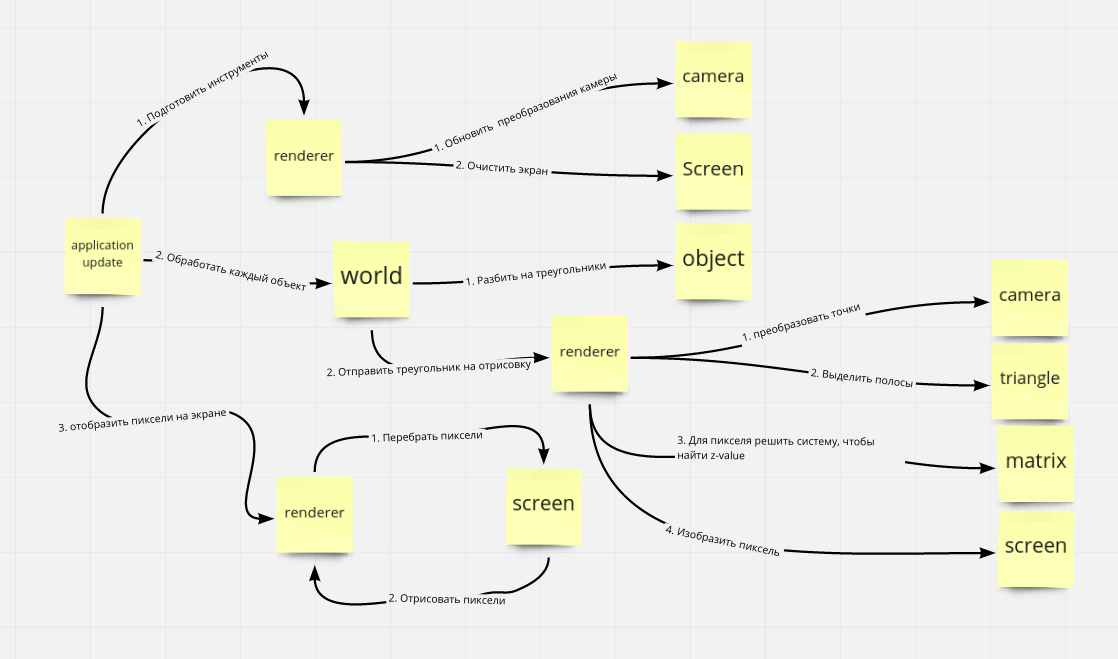
\includegraphics[width=0.6 \linewidth]{scheme_pipeline.png}

\end{center}

\begin{itemize}
\item Renderer
\item Camera
\item World
\item Window (SFML)
\end{itemize}

\end{frame}

\begin{frame}
\frametitle{Программная часть}

\begin{itemize}
\item Application --- тестовое приложение
\item Doxygen --- сопроводительная документация
\item CxxTest + Github Actions --- автоматические unit-тесты
\item GProf --- профайлер для исследования производительности
\end{itemize}
\end{frame}

\begin{frame}
\frametitle{Парсер .off-формата}

\begin{center}
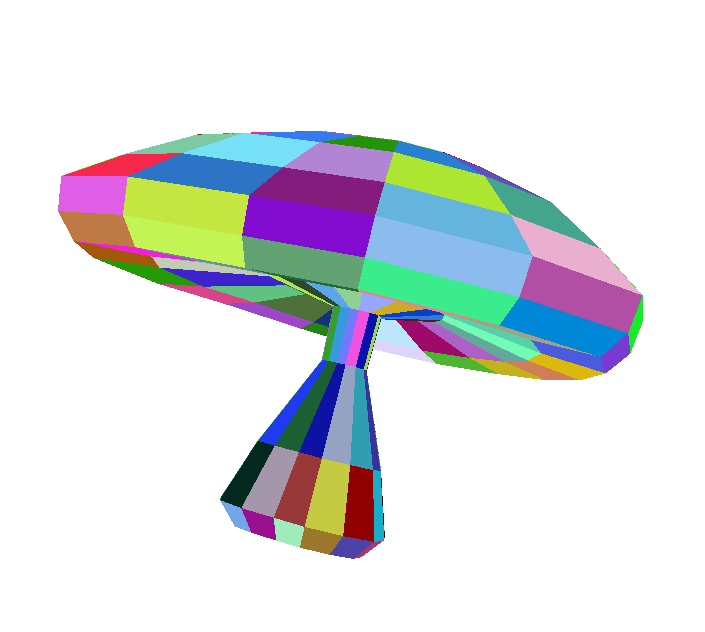
\includegraphics[width=3cm]{../example/mushroom.png}
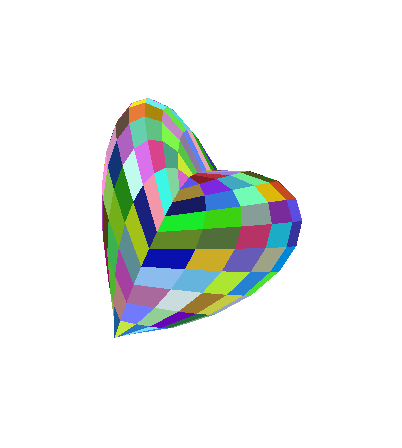
\includegraphics[width=3cm]{../example/heart.png}
\\
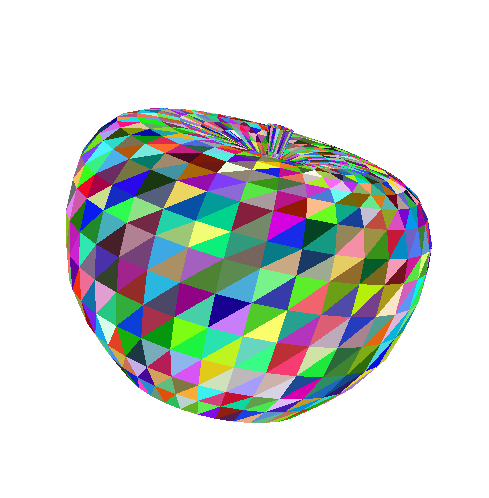
\includegraphics[width=3cm]{../example/apple.png}
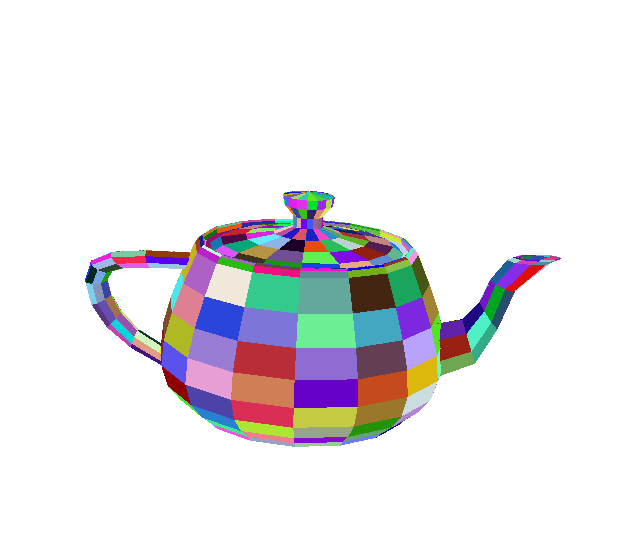
\includegraphics[width=3cm]{../example/teapot.png}
\end{center}
\end{frame}

\begin{frame}
\frametitle{Тени}

\begin{center}
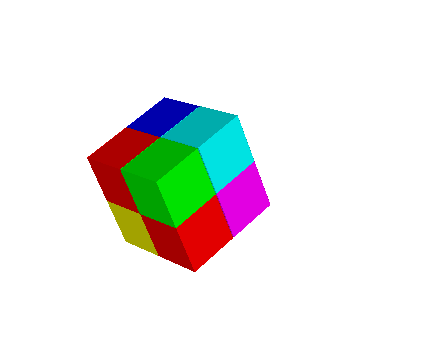
\includegraphics[width=0.5 \linewidth]{../example/cube_shadows.png}
\end{center}

Тень представляется как функция $\varphi:\ [0; 2\pi) \to [0; 1]$ от угла между направлением света и нормалью к плоскости, на которую домножается свет.

\end{frame}


\begin{frame}
\frametitle{Скорость работы}

\begin{itemize}
\item Согласно профилировщику GProf, большая часть времени уходит на процессы, связанные с растеризацией и пиксельным экраном.

\item 30\% производительности уходит непосредственно на методы \textit{Screen::validate\_pixel, Screen::set\_pixel}, и вспомогательные.

\item Кстати, во время разработки простой $x_{start} = \max(0, x_{start})$ заметно ускорил приложение.
\end{itemize}
\end{frame}

\begin{frame}
\frametitle{Результаты}

\begin{itemize}
\item Библиотека:
\begin{itemize}
	\item разработана
	\item протестирована
	\item задокументирована
\end{itemize}
\item Теория изучена
\item Приложение сделано
\item Дополнительно сделан парсинг 3d-моделей
\item Дополнительно сделаны тени
\end{itemize}
\end{frame}

\begin{frame}
\frametitle{3D-renderer с нуля}

\begin{center}
Спасибо за внимание!
\end{center}
\end{frame}


\end{document}
